% Aberdeen style guide should be followed when using this
% layout. Their template powerpoint slide is used to extract the
% Aberdeen color and logo but is otherwise ignored (it has little or
% no formatting in it anyway).
%
% http://www.abdn.ac.uk/documents/style-guide.pdf

%%%%%%%%%%%%%%%%%%%% Document Class Settings %%%%%%%%%%%%%%%%%%%%%%%%%
% Pick if you want slides, or draft slides (no animations)
%%%%%%%%%%%%%%%%%%%%%%%%%%%%%%%%%%%%%%%%%%%%%%%%%%%%%%%%%%%%%%%%%%%%%%
%Normal document mode
%\documentclass[10pt,compress]{beamer}
%Draft or handout mode
%\documentclass[10pt,compress,handout]{beamer}
\documentclass[10pt,compress,handout,ignorenonframetext]{beamer} 

%%%%%%%%%%%%%%%%%%%% General Document settings %%%%%%%%%%%%%%%%%%%%%%%
% These settings must be set for each presentation
%%%%%%%%%%%%%%%%%%%%%%%%%%%%%%%%%%%%%%%%%%%%%%%%%%%%%%%%%%%%%%%%%%%%%%
\newcommand{\shortname}{Dr Jeff Gomes} 
\newcommand{\fullname}{Dr Jeff Gomes}
\institute{School of Engineering}
\newcommand{\emailaddress}{}%{jefferson.gomes@abdn.ac.uk}
\newcommand{\logoimage}{./FigBanner/UoAHorizBanner}
\title{Computational Fluid Dynamics (EG501V)}
\subtitle{Module 01: Introduction to Computational Methods for Fluid Dynamics: Brief Overview of CFD Workflow}
\date[2015-16]{2015-16}


%%%%%%%%%%%%%%%%%%%% Template settings %%%%%%%%%%%%%%%%%%%%%%%%%%%%%%%
% You shouldn't have to change below this line, unless you want to.
%%%%%%%%%%%%%%%%%%%%%%%%%%%%%%%%%%%%%%%%%%%%%%%%%%%%%%%%%%%%%%%%%%%%%%
\usecolortheme{whale}
\useoutertheme{infolines}

% Use the fading effect for items that are covered on the current
% slide.
\beamertemplatetransparentcovered

% We abuse the author command to place all of the slide information on
% the title page.
\author[\shortname]{%
  \fullname\\\ttfamily{\emailaddress}
}


%At the start of every section, put a slide indicating the contents of the current section.
\AtBeginSection[] {
  \begin{frame}
    \frametitle{Section Outline}
    \tableofcontents[currentsection]
  \end{frame}
}

% Allow the inclusion of movies into the Presentation! At present,
% only the Okular program is capable of playing the movies *IN* the
% presentation.
\usepackage{multimedia}
\usepackage{animate}

%% Handsout -- comment out the lines below to create handstout with 4 slides in a page with space for comments
\usepackage{handoutWithNotes}

\mode<handout>
{
\usepackage{pgf,pgfpages}

\pgfpagesdeclarelayout{2 on 1 boxed with notes}
{
\edef\pgfpageoptionheight{\the\paperheight} 
\edef\pgfpageoptionwidth{\the\paperwidth}
\edef\pgfpageoptionborder{0pt}
}
{
\setkeys{pgfpagesuselayoutoption}{landscape}
\pgfpagesphysicalpageoptions
    {%
        logical pages=4,%
        physical height=\pgfpageoptionheight,%
        physical width=\pgfpageoptionwidth,%
        last logical shipout=2%
    } 
\pgfpageslogicalpageoptions{1}
    {%
    border code=\pgfsetlinewidth{1pt}\pgfstroke,%
    scale=1,
    center=\pgfpoint{.25\pgfphysicalwidth}{.75\pgfphysicalheight}%
    }%
\pgfpageslogicalpageoptions{2}
    {%
    border code=\pgfsetlinewidth{1pt}\pgfstroke,%
    scale=1,
    center=\pgfpoint{.25\pgfphysicalwidth}{.25\pgfphysicalheight}%
    }%
\pgfpageslogicalpageoptions{3}
    {%
    border shrink=\pgfpageoptionborder,%
    resized width=.7\pgfphysicalwidth,%
    resized height=.5\pgfphysicalheight,%
    center=\pgfpoint{.75\pgfphysicalwidth}{.29\pgfphysicalheight},%
    copy from=3
    }%
\pgfpageslogicalpageoptions{4}
    {%
    border shrink=\pgfpageoptionborder,%
    resized width=.7\pgfphysicalwidth,%
    resized height=.5\pgfphysicalheight,%
    center=\pgfpoint{.75\pgfphysicalwidth}{.79\pgfphysicalheight},%
    copy from=4
    }%

\AtBeginDocument
    {
    \newbox\notesbox
    \setbox\notesbox=\vbox
        {
            \hsize=\paperwidth
            \vskip-1in\hskip-1in\vbox
            {
                \vskip1cm
                Notes\vskip1cm
                        \hrule width\paperwidth\vskip1cm
                    \hrule width\paperwidth\vskip1cm
                        \hrule width\paperwidth\vskip1cm
                    \hrule width\paperwidth\vskip1cm
                        \hrule width\paperwidth\vskip1cm
                    \hrule width\paperwidth\vskip1cm
                    \hrule width\paperwidth\vskip1cm
                    \hrule width\paperwidth\vskip1cm
                        \hrule width\paperwidth
            }
        }
        \pgfpagesshipoutlogicalpage{3}\copy\notesbox
        \pgfpagesshipoutlogicalpage{4}\copy\notesbox
    }
}
}

%\pgfpagesuselayout{2 on 1 boxed with notes}[letterpaper,border shrink=5mm]
%\pgfpagesuselayout{2 on 1 boxed with notes}[letterpaper,border shrink=5mm]

%%%%% Color settings
\usepackage{color}
%% The background color for code listings (i.e. example programs)
\definecolor{lbcolor}{rgb}{0.9,0.9,0.9}%
\definecolor{UoARed}{rgb}{0.64706, 0.0, 0.12941}
\definecolor{UoALight}{rgb}{0.85, 0.85, 0.85}
\definecolor{UoALighter}{rgb}{0.92, 0.92, 0.92}
\setbeamercolor{structure}{fg=UoARed} % General background and higlight color
\setbeamercolor{frametitle}{bg=black} % General color
\setbeamercolor{frametitle right}{bg=black} % General color
\setbeamercolor{block body}{bg=UoALighter} % For blocks
\setbeamercolor{structure}{bg=UoALight} % For blocks
% Rounded boxes for blocks
\setbeamertemplate{blocks}[rounded]

%%%%% Font settings
% Aberdeen requires the use of Arial in slides. We can use the
% Helvetica font as its widely available like so
% \usepackage{helvet}
% \renewcommand{\familydefault}{\sfdefault}
% But beamer already uses a sans font, so we will stick with that.

% The size of the font used for the code listings.
\newcommand{\goodsize}{\fontsize{6}{7}\selectfont}

% Extra math packages, symbols and colors. If you're using Latex you
% must be using it for formatting the math!
\usepackage{amscd,amssymb} \usepackage{amsfonts}
\usepackage[mathscr]{eucal} \usepackage{mathrsfs}
\usepackage{latexsym} \usepackage{amsmath} \usepackage{bm}
\usepackage{amsthm} \usepackage{textcomp} \usepackage{eurosym}
% This package provides \cancel{a} and \cancelto{a}{b} to "cancel"
% expressions in math.
\usepackage{cancel}

\usepackage{comment} 

% Get rid of font warnings as modern LaTaX installations have scalable
% fonts
\usepackage{type1cm} 

%\usepackage{enumitem} % continuous numbering throughout enumerate commands

% For exact placement of images/text on the cover page
\usepackage[absolute]{textpos}
\setlength{\TPHorizModule}{1mm}%sets the textpos unit
\setlength{\TPVertModule}{\TPHorizModule} 

% Source code formatting package
\usepackage{listings}%
\lstset{ backgroundcolor=\color{lbcolor}, tabsize=4,
  numberstyle=\tiny, rulecolor=, language=C++, basicstyle=\goodsize,
  upquote=true, aboveskip={1.5\baselineskip}, columns=fixed,
  showstringspaces=false, extendedchars=true, breaklines=false,
  prebreak = \raisebox{0ex}[0ex][0ex]{\ensuremath{\hookleftarrow}},
  frame=single, showtabs=false, showspaces=false,
  showstringspaces=false, identifierstyle=\ttfamily,
  keywordstyle=\color[rgb]{0,0,1},
  commentstyle=\color[rgb]{0.133,0.545,0.133},
  stringstyle=\color[rgb]{0.627,0.126,0.941}}

% Allows the inclusion of other PDF's into the final PDF. Great for
% attaching tutorial sheets etc.
\usepackage{pdfpages}
\setbeamercolor{background canvas}{bg=}  

% Remove foot note horizontal rules, they occupy too much space on the slide
\renewcommand{\footnoterule}{}

% Force the driver to fix the colors on PDF's which include mixed
% colorspaces and transparency.
\pdfpageattr {/Group << /S /Transparency /I true /CS /DeviceRGB>>}

% Include a graphics, reserve space for it but
% show it on the next frame.
% Parameters:
% #1 Which slide you want it on
% #2 Previous slides
% #3 Options to \includegraphics (optional)
% #4 Name of graphic
\newcommand{\reserveandshow}[4]{%
\phantom{\includegraphics<#2|handout:0>[#3]{#4}}%
\includegraphics<#1>[#3]{#4}%
}

\newcommand{\frc}{\displaystyle\frac}
\newcommand{\red}{\textcolor{red}}
\newcommand{\blue}{\textcolor{blue}}
\newcommand{\green}{\textcolor{green}}
\newcommand{\purple}{\textcolor{purple}}
 

\begin{document}

% Title page layout
\begin{frame}
  \titlepage
  \vfill%
  \begin{center}
    \includegraphics[clip,width=0.8\textwidth]{\logoimage}
  \end{center}
\end{frame}

% Table of contents
%\frame{ \frametitle{Slides Outline}
%  \tableofcontents
%}


%%%%%%%%%%%%%%%%%%%% The Presentation Proper %%%%%%%%%%%%%%%%%%%%%%%%%
% Fill below this line with \begin{frame} commands! It's best to
% always add the fragile option incase you're going to use the
% verbatim environment.
%%%%%%%%%%%%%%%%%%%%%%%%%%%%%%%%%%%%%%%%%%%%%%%%%%%%%%%%%%%%%%%%%%%%%%



%%%%%%%%%%%%%%%%%%%
%%%   SECTION   %%%
%%%%%%%%%%%%%%%%%%%
\section{Workflow for Computational Fluid Dynamics (CFD) Simulations}

%##################
%%%   SUBSECTION
%##################
\subsection{Motivation}
%%%
%%% Slide
%%%
\begin{frame}
 \frametitle{Initial Definition}

\begin{enumerate}
\item <1->\textcolor{blue}{Computational Fluid Dynamics (CFD)} is a numerical tool to predict (qualitatively and quantitatively) fluid flow using:
\begin{enumerate}
\item <2-> Mathematical modelling $\rightarrow$ representing the physics by partial differential equations (PDE);
\item <3-> Numerical methods $\rightarrow$ set of discretisation and solution techniques for the PDE and;
\item <4-> Software tools $\rightarrow$ set of solvers, pre- and post-processing technologies.
\end{enumerate}
\item <5-> \textcolor{blue}{Numerical simulations} produced by CFD models can be seen as $\lq$Virtual Fluid Flow Laboratory';
\item <6-> \textcolor{blue}{CFD} is more cost-effective (i.e., less financially expansive) than experimental testing;
\item <7-> \textcolor{blue}{CFD} has been used to:
\begin{enumerate}
\item <8-> Improve the understanding of the fluid flow and potential interactions with solids (e.g., internal structures), chemical reactions, etc;
\item <9-> Assess the performance of equipment / facilities;
\item <10-> Aid in the design of new equipment / facilities;
\item <11-> Identify potential operational problems (e.g., safety assessment of industrial processes);
\item <12-> Guide experiments.
\end{enumerate}

\end{enumerate}
 
\end{frame}

%%%
%%% Slide
%%%
\begin{frame}
 \frametitle{Field Observation, Experiments and Numerical Simulations} 

   \begin{figure}%
    \begin{center}
     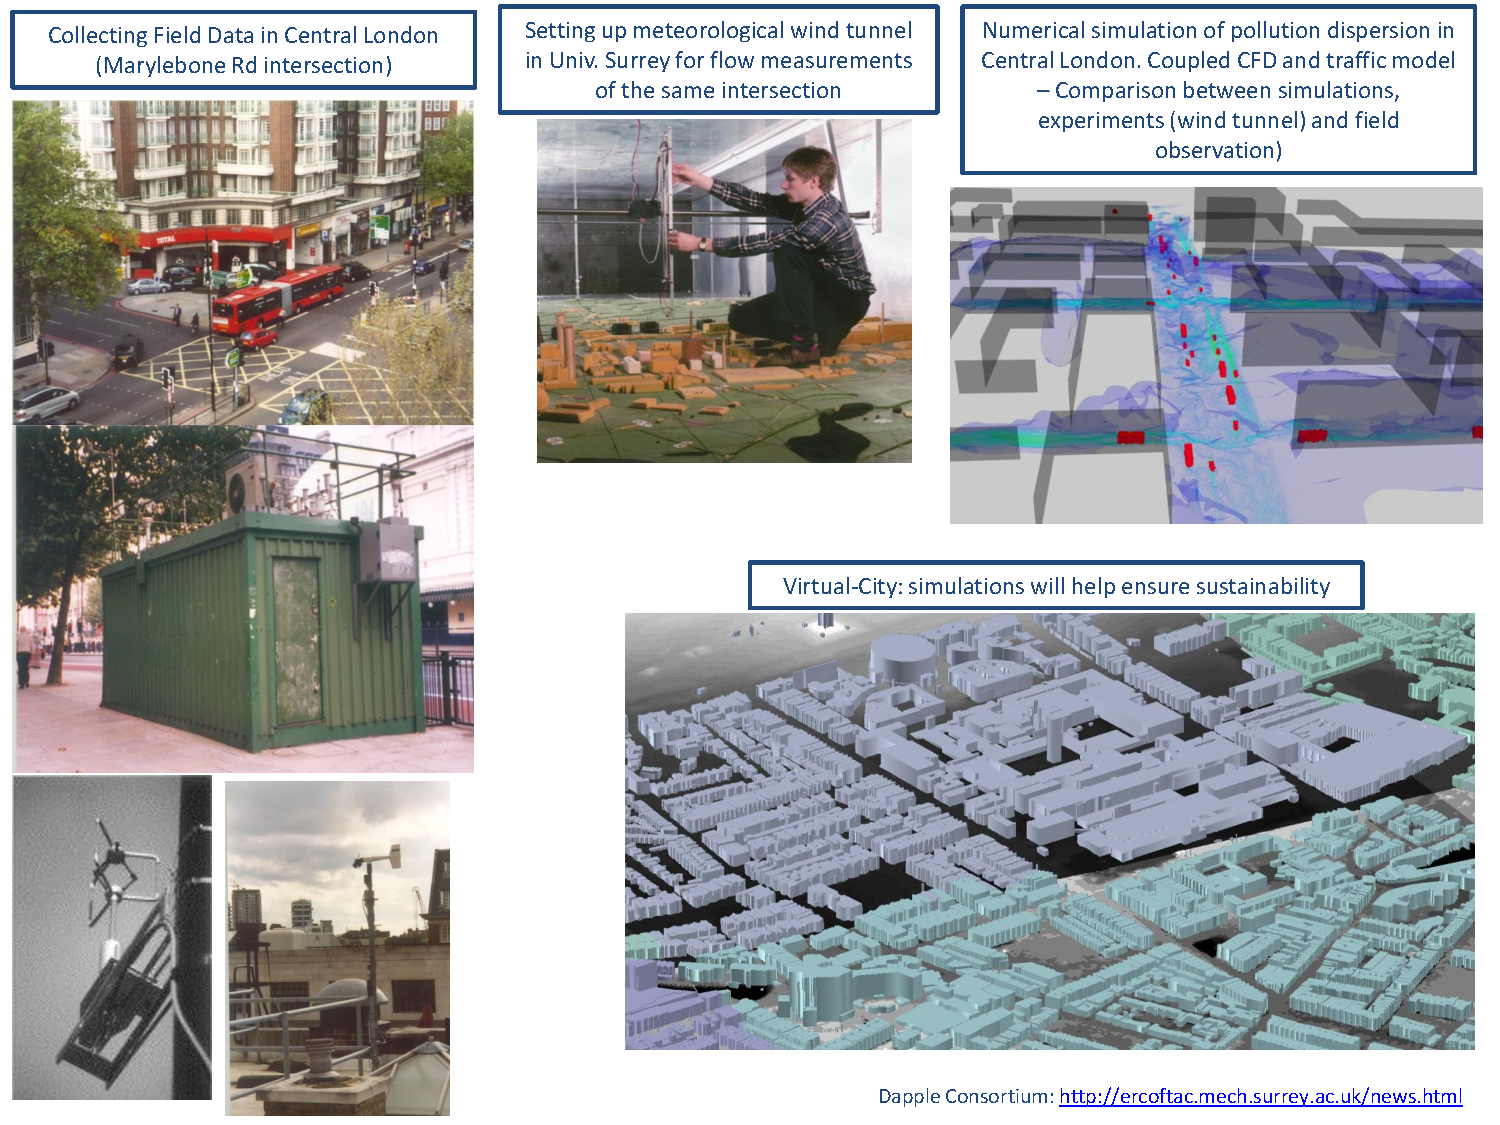
\includegraphics[width=12.cm, height=7.8cm, clip]{./Figs/Dapple.pdf}
    \end{center}
%\caption{XX}
   \end{figure}    

\end{frame}

%%%
%%% Slide
%%%
\begin{frame}
 \frametitle{Main Applications} 
\begin{enumerate}
\item <1-> Environmental Flows:
  \begin{enumerate}
    \item <2-> Flow circulation (and cycles) in ocean, rivers, lakes etc;
    \item <3-> Weather forecasting;
    \item <4-> Pyroclastic flows (volcanoes), avalanches, landslides, etc;
    \item <5-> Floodings, fire (e.g., forests), aquifers etc.
  \end{enumerate}
\item <6-> Industrial Flows:
  \begin{enumerate}
    \item <7-> Aerospace;
    \item <8-> Chemical processing;
    \item <9-> Power generation (eg.g., nuclear reactors, NG and coal-fire power stations, wind turbines, etc);
    \item <10-> Automotive;
    \item <11-> Oil and gas, etc. 
  \end{enumerate}
\item <12-> Biomedical engineering (e.g., cardiovascular systems);
\item <13-> etc.
  
\end{enumerate}

\end{frame}


%%%
%%% Slide
%%%
\begin{frame}
 \frametitle{Environmental Flows} 

   \begin{figure}%
    \begin{center}
     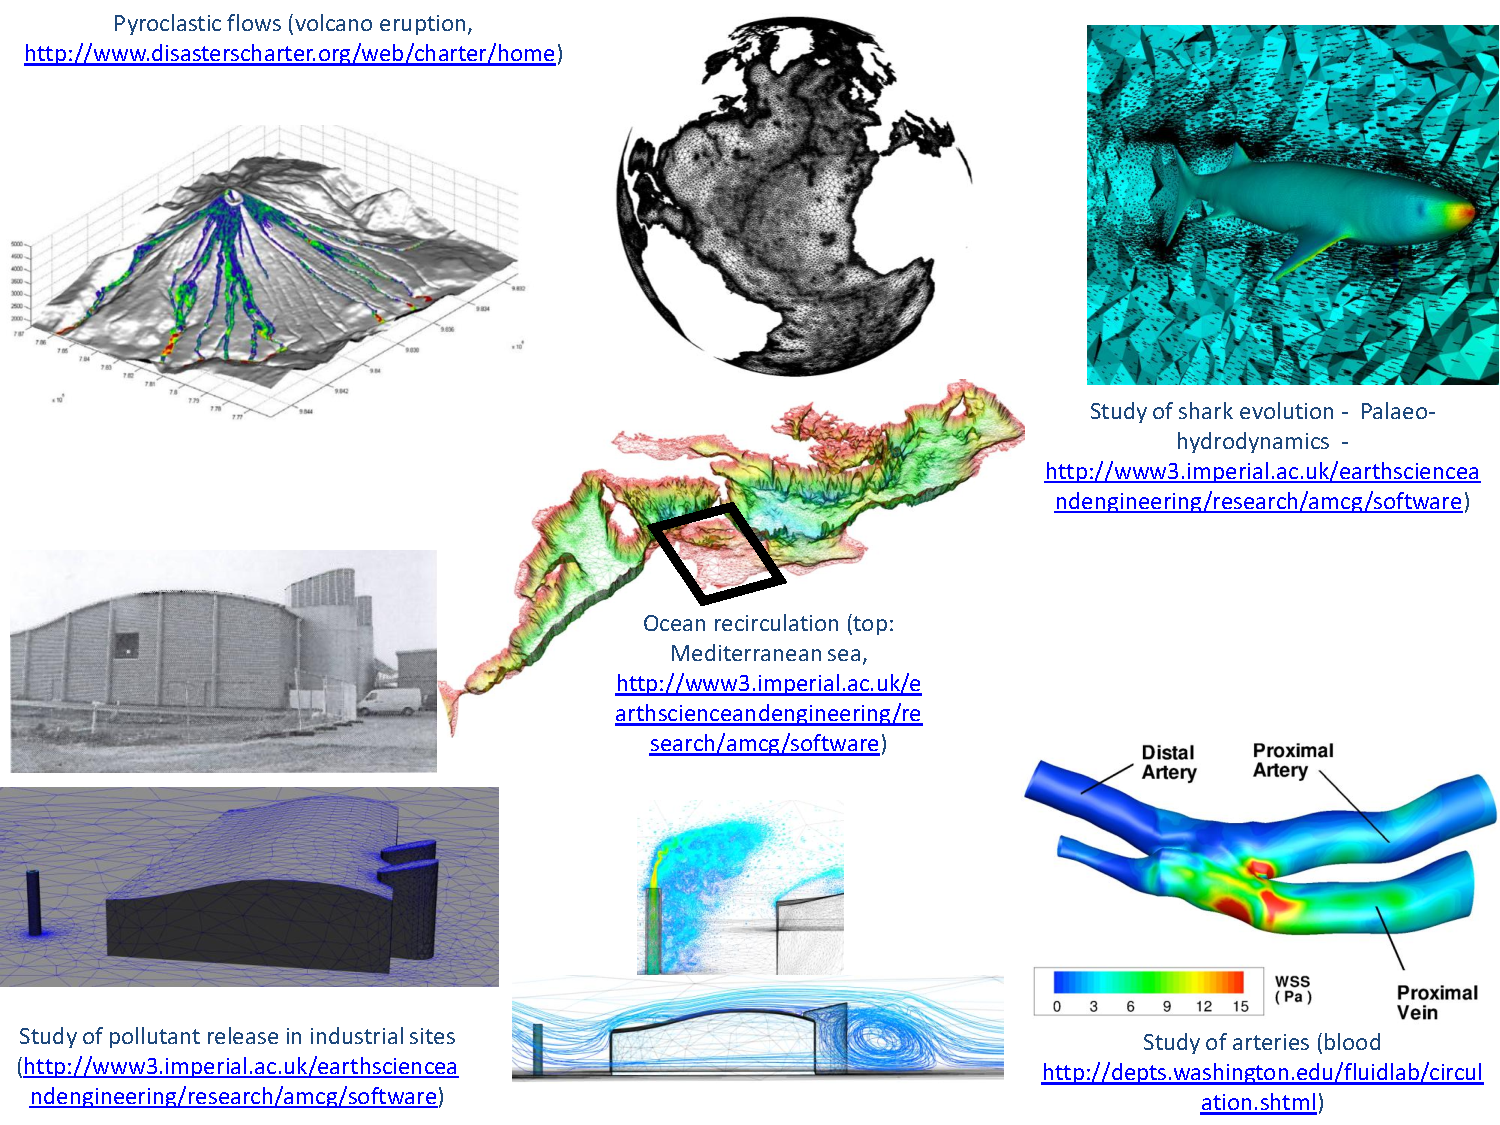
\includegraphics[width=12.cm, height=7.8cm, clip]{./Figs/EnvironmentallApplications.pdf}
    \end{center}
%\caption{XX}
   \end{figure}    

\end{frame}

%%%
%%% Slide
%%%
\begin{frame}
 \frametitle{Industrial Flows} 

   \begin{figure}%
    \begin{center}
     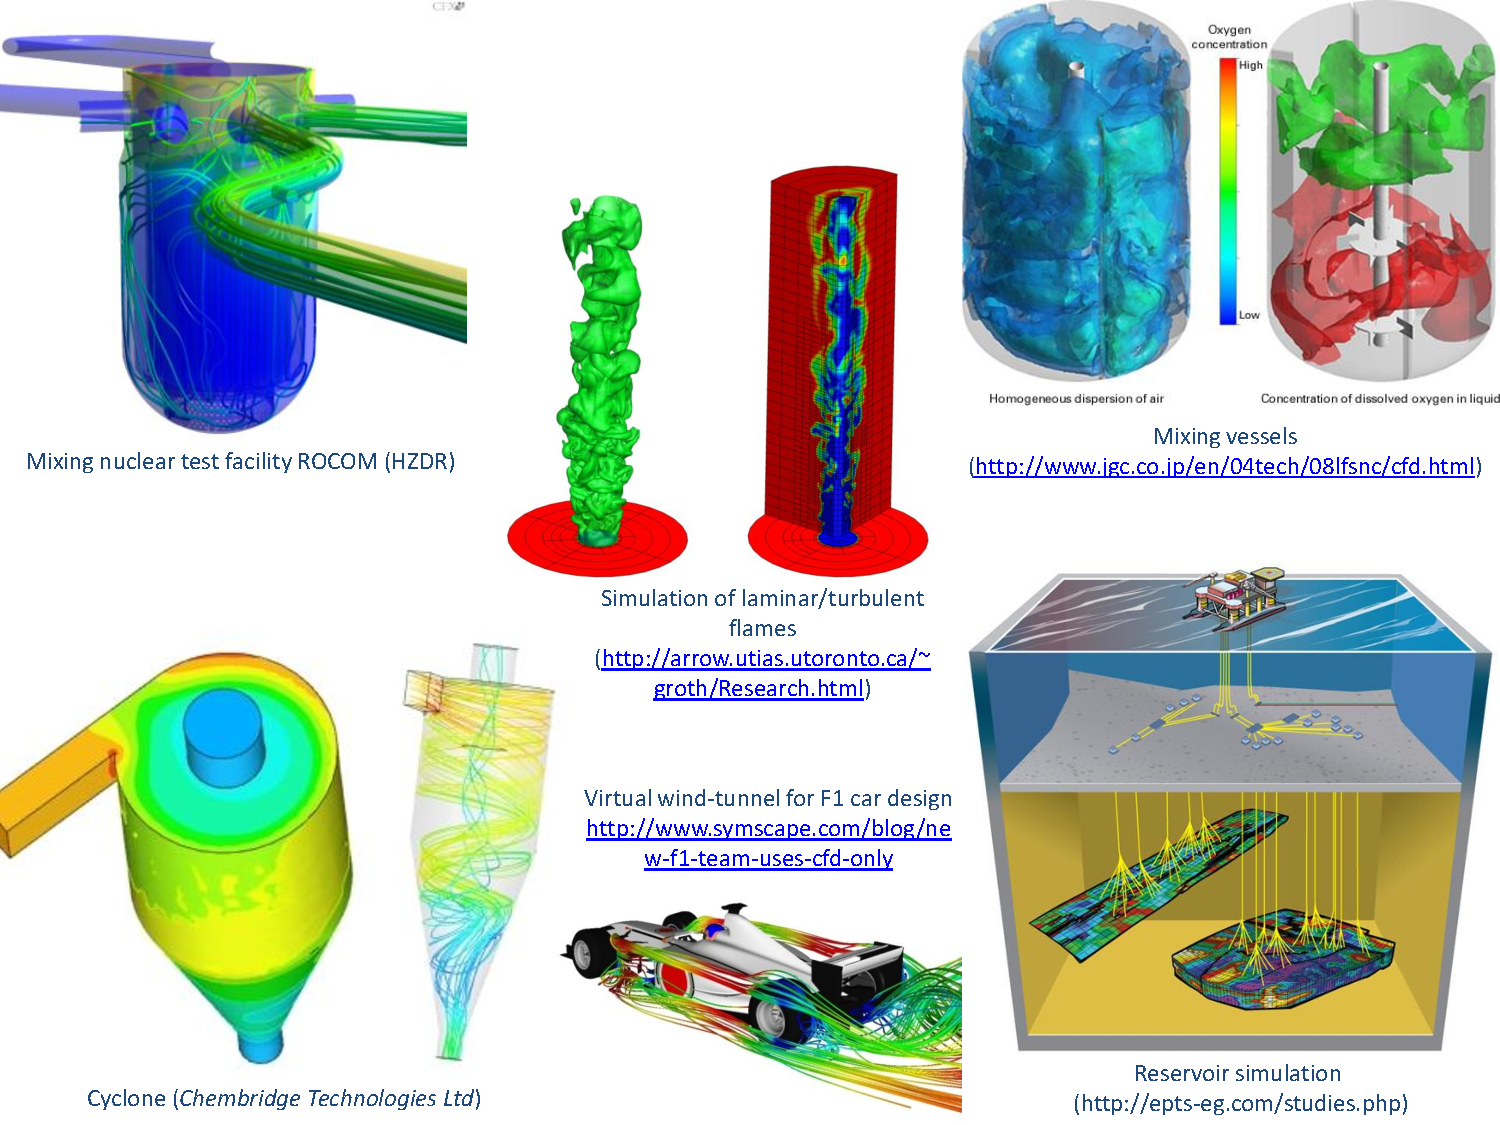
\includegraphics[width=12.cm, height=7.8cm, clip]{./Figs/IndustrialApplications.pdf}
    \end{center}
%\caption{XX}
   \end{figure}    

\end{frame}


%##################
%%%   SUBSECTION
%##################
\subsection{CFD Workflow}
 
%%%
%%% Slide
%%%
\begin{frame}
 \frametitle{Overview: Preprocessing} 
\begin{enumerate}
  \item <1-> We start with a mathematical model that represents a physical system, via:
    \begin{enumerate}
      \item <2-> Mass, momentum and energy conservative equations (e.g., Navier-Stokes, Stokes, Darcy, Richards equations, etc);
      \item <3-> Parametrisation of system properties (e.g., equations of state to define fluid densities, algebraic expressions for viscosities, thermal conductivity, etc);
      \item <4-> General simplifying assumptions (e.g., inviscid / viscous, steady-state / transient, laminar / turbulent, 1-/2-/3-D, compressible/incompressible, etc); 
      \item <5-> Appropriate set of boundary and initial conditions.
    \end{enumerate}
  \item <6-> Discretise the geometry (mathematical domain) with mesh/grids containing cells (or elements or control volumes): 
    \begin{enumerate}
      \item <7-> 2-D: Triangle and quadrilateral;
      \item <8-> 3-D: Tetrahedron, hexahedron, pyramid, prism with triangular base, etc 
    \end{enumerate}
\end{enumerate} 
\begin{itemize}
   \item <9-> The mesh/grid can either be structured (i.e., regular connectivity), unstructured (i.e., irregular connectivity) and hybrid;
   \item <10-> The stage of: (a) designing the geometry that represents the physical problem, (b) meshing the designed geometry; (c) input initial and boundary conditions; (d) prescribed operation conditions and (e) solver options \textcolor{red}{$\Longrightarrow$} is also called \textcolor{blue}{\underline{Preprocessing}}.
\end{itemize}  

\end{frame} 

%%%
%%% Slide
%%%
\begin{frame}
 \frametitle{Overview: Mesh Grid Classification}

   \begin{figure}%
    \begin{center}
     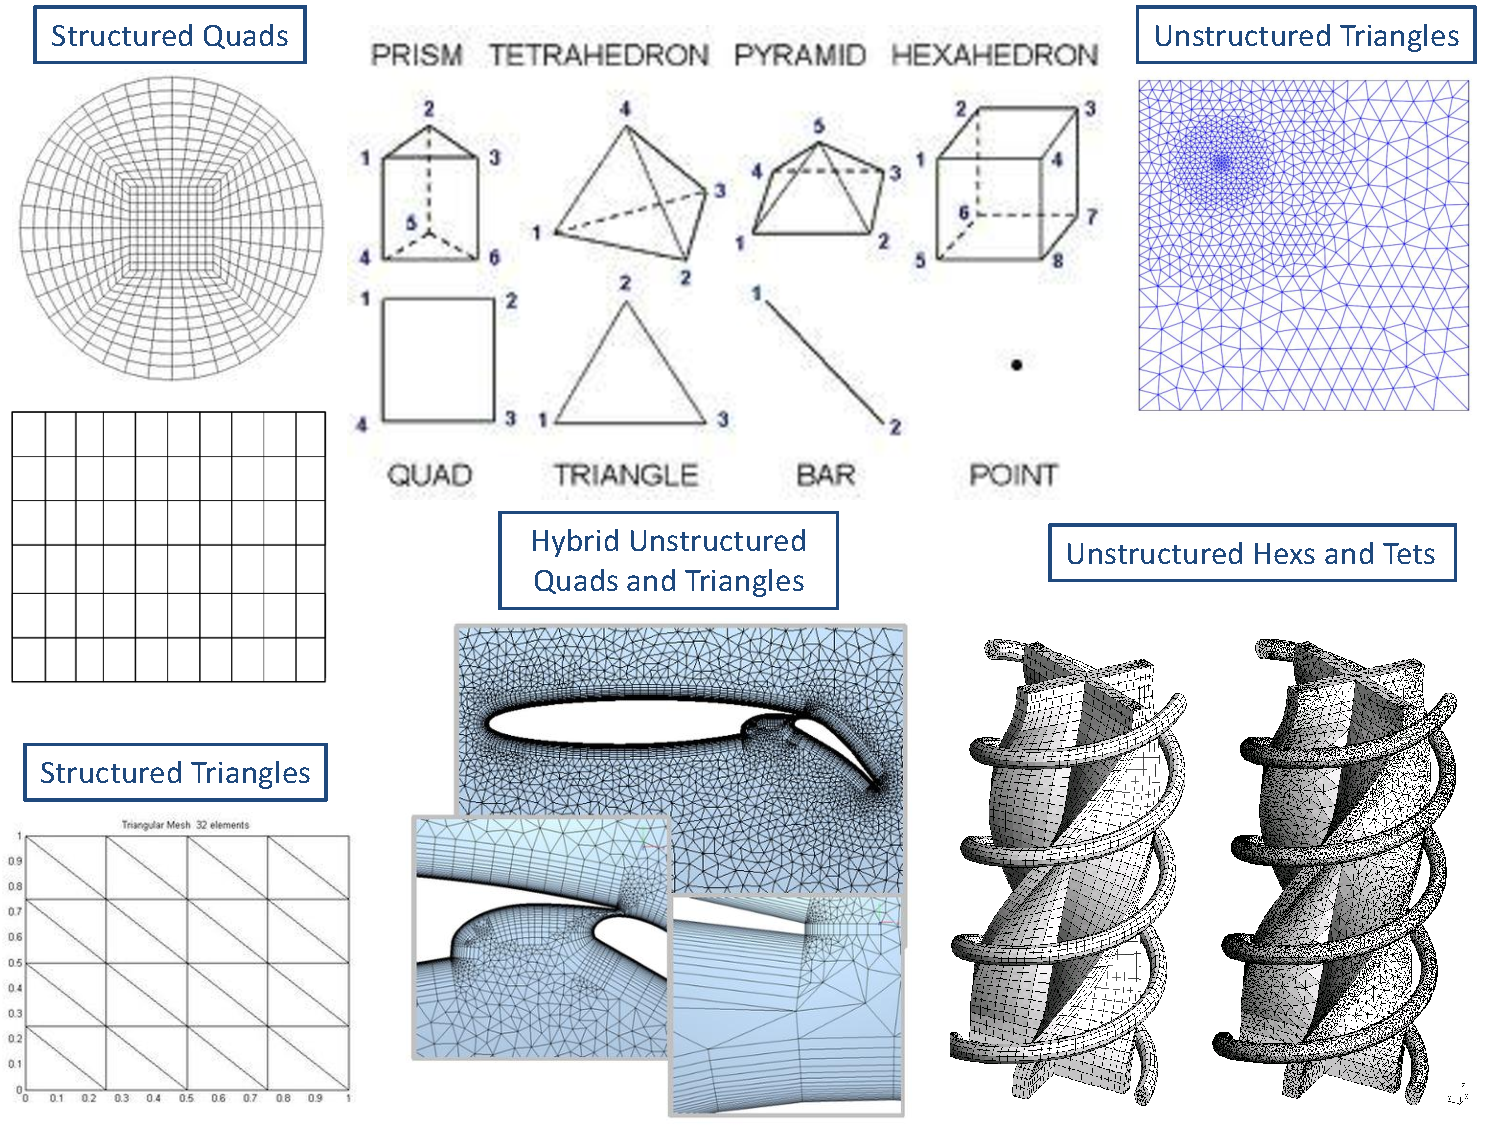
\includegraphics[width=12.cm, height=7.8cm, clip]{./Figs/MeshGrid_Examples.pdf}\label{xx}
    \end{center}
%\caption{XX}
   \end{figure}    

\end{frame}

%%%
%%% Slide
%%% 
\begin{frame}
 \frametitle{Overview: Discretisation Methods} 
\begin{enumerate}
  \setcounter{enumi}{2}
  \item <1-> Discretisation of the governing equations splitting into:
    \begin{enumerate}
      \item <2-> Space discretisation:
        \begin{enumerate}
          \item <4-> Finite difference methods (FDM); 
          \item <5-> Finite element methods (FEM); 
          \item <6-> Finite volume methods (FVM); 
          \item <7-> Boundary element methods (BEM); 
          \item <8-> Spectral element methods (SEM); 
          \item <9-> Spectral finite element methods (SFEM); 
          \item <10-> etc. 
        \end{enumerate}
      \item <3-> Time discretisation:
        \begin{enumerate}
          \item <11-> Explicit Methods: Forward-Euler, Leapfrog, etc;
          \item <12-> Implicit Methods: Backward-Euler, Crank-Nicolson, etc;
          \item <13-> Hybrid Methods: $\lq$family' of Runge-Kutta methods.
        \end{enumerate}
    \end{enumerate}
\end{enumerate}
\end{frame}


%%%
%%% Slide
%%% 
\begin{frame}
 \frametitle{Overview: Discretisation Methods} 
\begin{enumerate}
  \setcounter{enumi}{3}
  \item <1-> The conservative partial differential equations after the coupled time- and spatial-discretisation become algebraic equations;
  \item <2-> This set of algebraic linear equations are manipulated to become, in the matricial form:
    \visible<2->{
      \begin{equation}
         \underline{\underline{A}}\;\underline{x}=\underline{b}\label{Eq:LinearEqns}
      \end{equation}}
      \begin{enumerate}
         \item<3-> The components of matrix \textcolor{blue}{$\underline{\underline{A}}$ $\left(a_{ij}\right)$} are related to nodes and elements/cells for all conservative equations (i.e., continuity, momentum and energy) and constitutive relations (i.e., EOS, viscosity correlations etc);
         \item<4-> \textcolor{blue}{$\underline{x}$} is solution-vector of the system of linear equations (e.g., velocity, pressure, temperature, concentration etc);
         \item <5-> The vector \textcolor{blue}{$\underline{b}$} corresponds to the remaining terms of the right-hand side of the conservative equations.
      \end{enumerate}
\end{enumerate}

\end{frame}


%%%
%%% Slide
%%% 
\begin{frame}
 \frametitle{Overview: Linear Solvers} 
\begin{enumerate}
  \setcounter{enumi}{5}
  \item <1-> The system of linear equations (Eqn.~\ref{Eq:LinearEqns}) are solved simultaneously to obtain \textcolor{blue}{$\underline{x}$};
  \item <2-> Several methods were developed to solve this system of equations, e.g.,
    \begin{enumerate}
       \item<3-> Direct Methods: 
          \begin{enumerate}
             \item <5-> Gauss-Elimination;
             \item <6-> Lower-Upper (LU) decomposition / factorisation;
             \item <7-> Tridiagonal matrix algorithm (TDMA);
             \item <8-> etc. 
          \end{enumerate}
       \item<4-> Iterative Methods:
          \begin{enumerate}
             \item <9-> Jacobi;
             \item <10-> Gauss-Seidel;
             \item <11-> Successive Over-Relaxation (SOR);
             \item <12-> Conjugate Gradient methods;
             \item <13-> Multigrid Methods;
             \item <14-> etc.
          \end{enumerate}
    \end{enumerate}
  \item <15-> For realistic (i.e., large) CFD calculations, iterative methods are {\bf always} used. However, direct methods can also be used as $\lq$preconditioning methods' for the system of equations;
   \item <16-> A large number of iterations are often required to reach a converged solution, i.e., changes in the \textcolor{blue}{solution-vector $\left(\underline{x}\right)$} between two continuous iterations are smaller than prescribed \underline{tolerances}.
\end{enumerate}

\end{frame}
 

%%%
%%% Slide
%%% 
\begin{frame}
 \frametitle{Overview: Post-Processing} 
\begin{enumerate}
  \setcounter{enumi}{9}
  \item <1-> Visualisation (snapshots and time-series) can help to:
      \begin{enumerate}
         \item <2-> Identify flow patterns (e.g., bubbles, flow regimes, temperature profiles etc);
         \item <3-> Investigate how specific calculated fields evolves in time and space (e.g., temperature, velocities pressure etc);
         \item <4-> Ensure that initial and boundary conditions are correctly imposed;
         \item <5-> Investigate diagnostic fields, i.e., variables that are calculated from or along with field-solutions. E.g., local and averaged drag, lift and heat transfer coefficients, mass/volumetric fluxes etc;
      \end{enumerate}
  \item <6-> Most CFD software have (either as native or third-party) embedded diagnostic tools for:
      \begin{enumerate}
         \item <7-> Grid, contour, vector plots;
         \item <8-> Pathline trajectory and XY plots;
         \item <9-> Animations;
         \item <10-> Surface and volume integrals and averages;
         \item <11-> Power spectral density (PSD), Fast Fourier transform (FFT) and other statistical tools;
         \item <12-> Forces and moments;
         \item <13-> etc.
      \end{enumerate}

\end{enumerate}

\end{frame}
 
%%%
%%% Slide
%%%
\begin{frame}
 \frametitle{Overview: Post-Processing}

   \begin{figure}%
    \begin{center}
     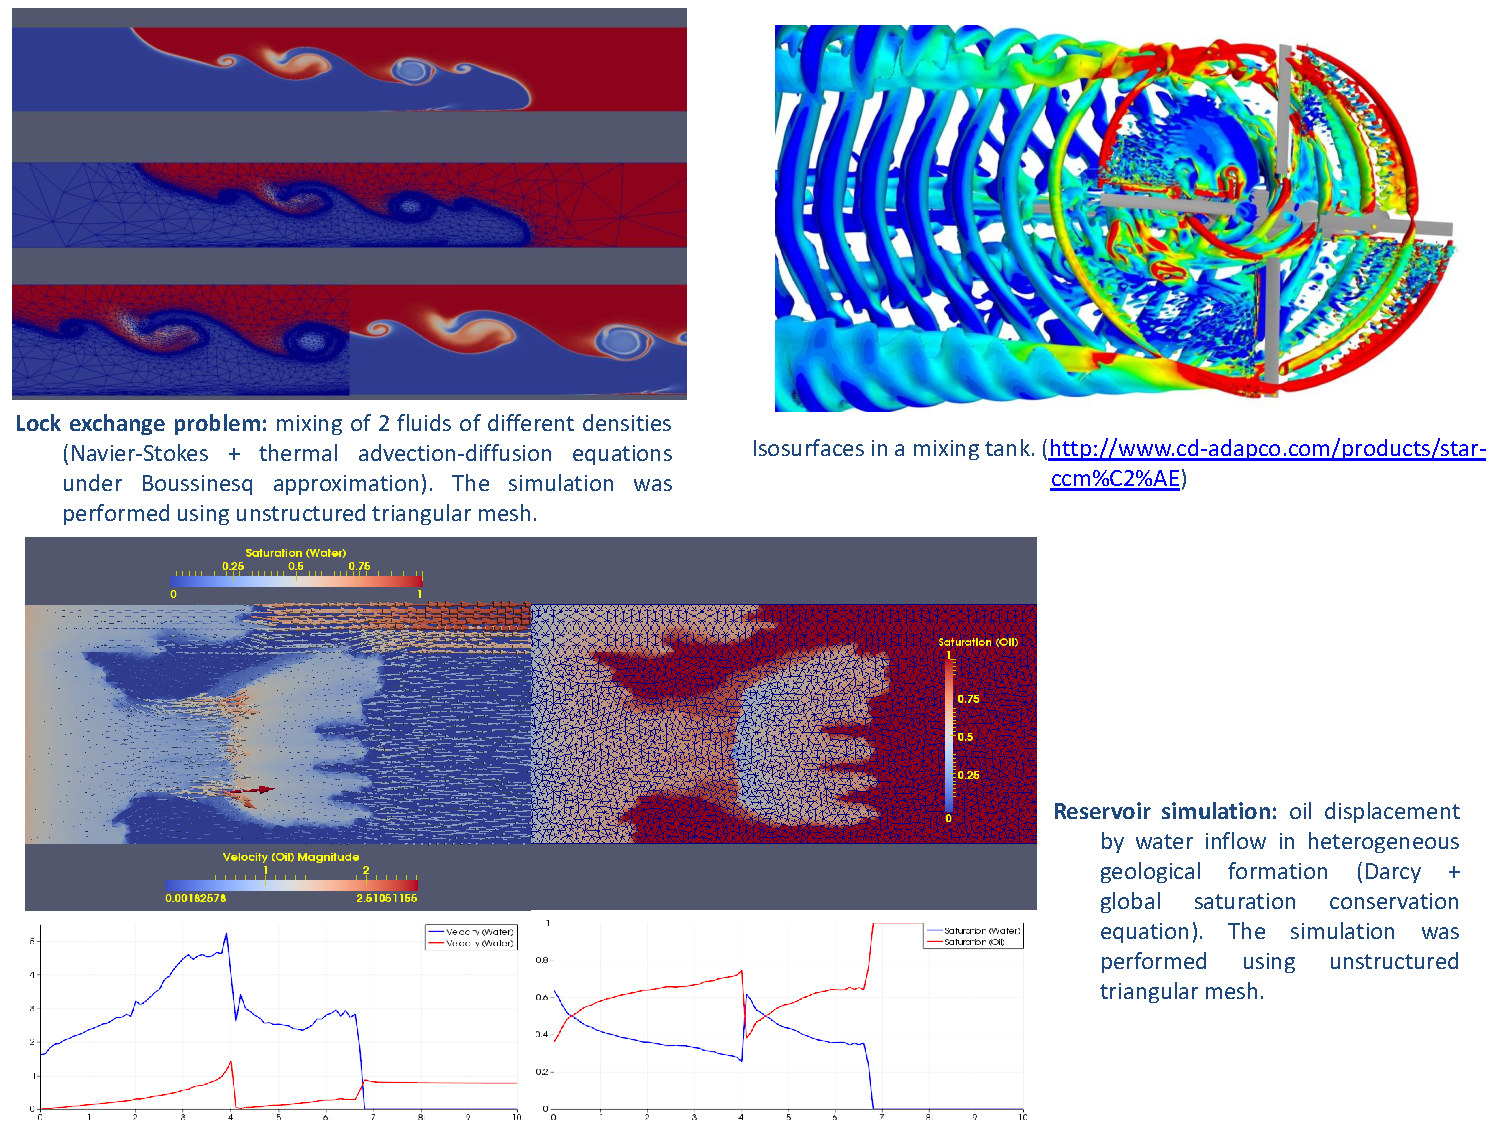
\includegraphics[width=12.cm, height=7.8cm, clip]{./Figs/PostProcessingExamples.pdf}
    \end{center}
%\caption{XX}
   \end{figure}    

\end{frame}

%%%
%%% Slide
%%%
\begin{frame}
 \frametitle{Example: Pollution dispersion in an industrial site}

   \begin{figure}%
    \begin{center}
     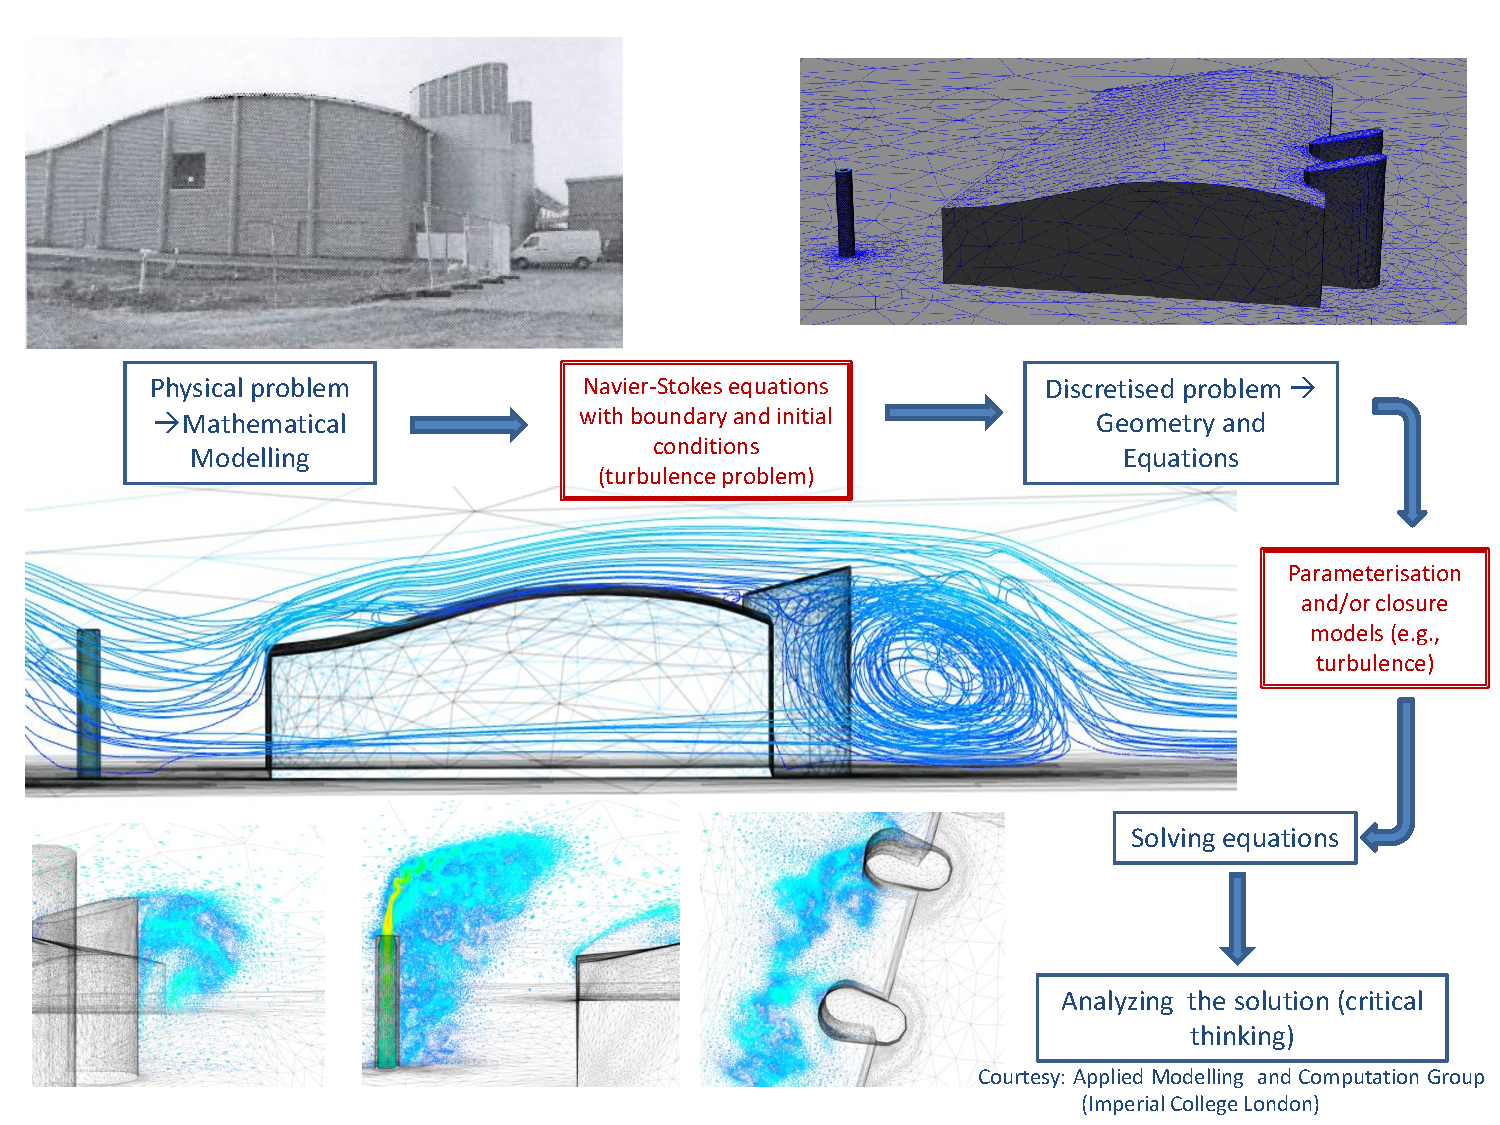
\includegraphics[width=12.cm, height=7.8cm, clip]{./Figs/SpecificIndustrialEnvironmentalApplication.pdf}
    \end{center}
%\caption{XX}
   \end{figure}    

\end{frame}


%%%
%%% Slide
%%%
\begin{frame}
 \frametitle{Overview: Workflow}

   \begin{figure}%
    \begin{center}
     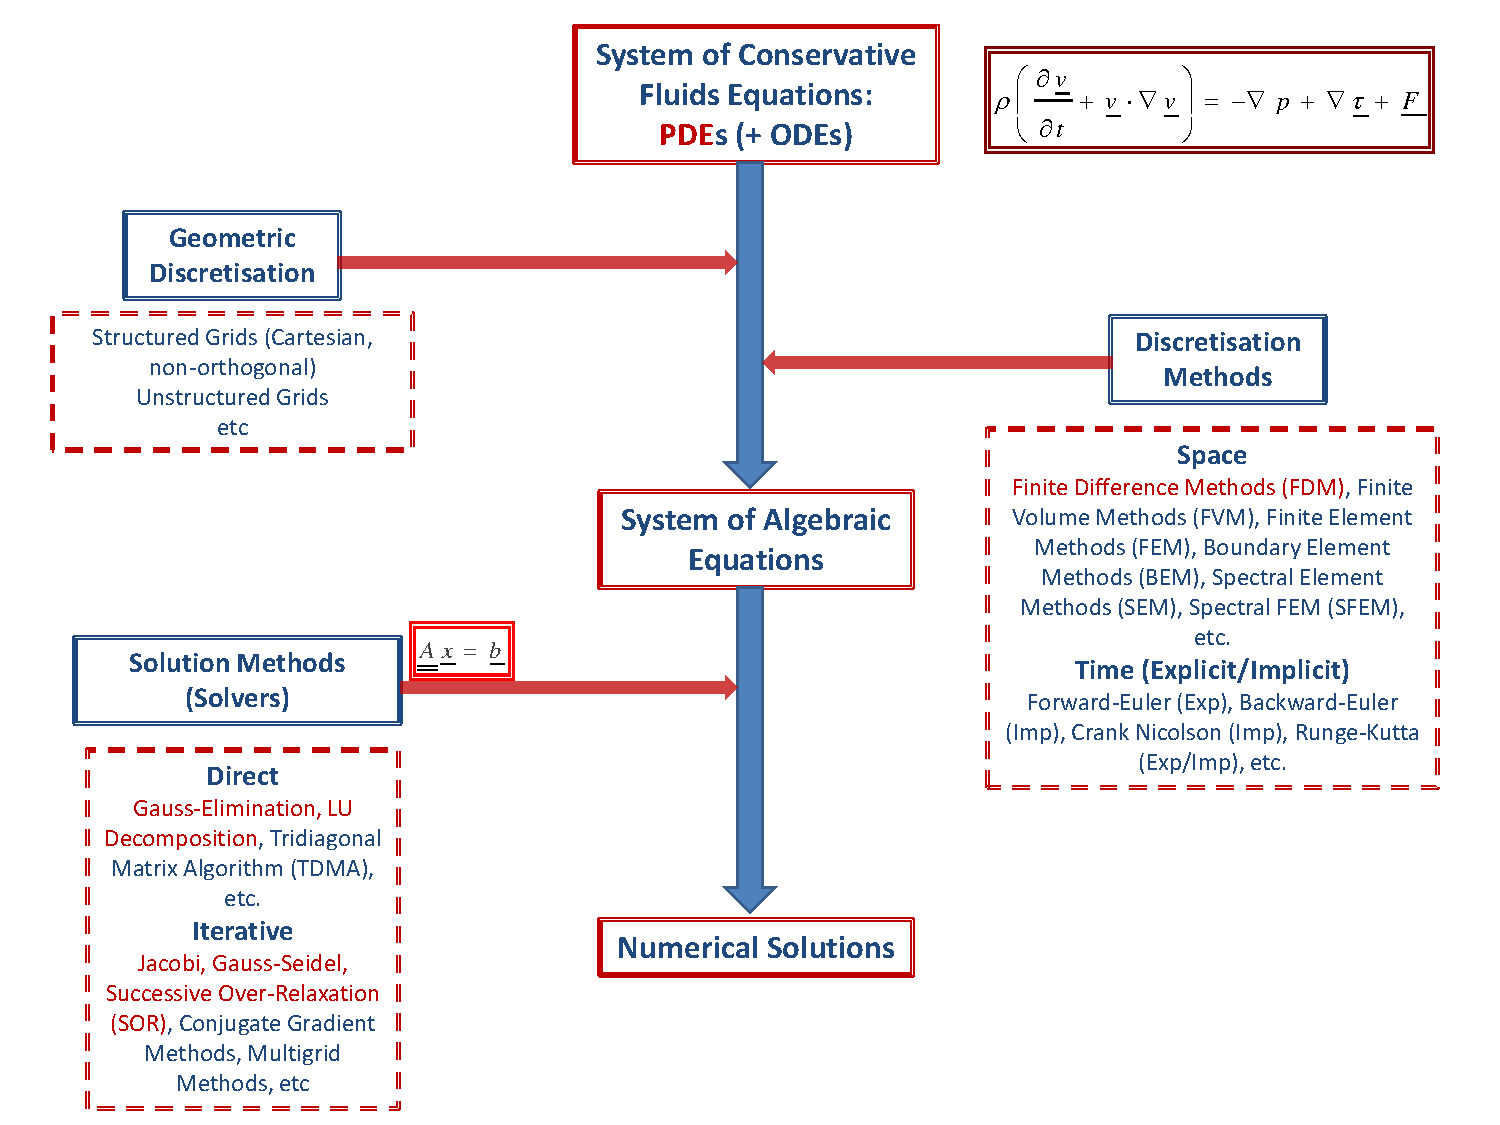
\includegraphics[width=12.cm, height=7.8cm, clip]{./Figs/CFD_Schematics2.pdf}
    \end{center}
%\caption{XX}
   \end{figure}    

\end{frame}

\subsection{A few available CFD}  
%%%
%%% Slide
%%%
\begin{frame}
 \frametitle{Common Flow Simulators}
\begin{center}
\begin{tabular}{||c|| c | c | c | c ||}
\hline\hline
                   & {\bf Type}  & 
{\bf Mesh}\footnote{S: Structured, U: Unstructured, T: Triangle / Tetrahedral, Q: Quadrilateral / Hexahedral, H: Hybrids, A: All.} & 
{\bf Problem}\footnote{Single phase and multiphase fluid flows.} & 
{\bf Solution}\footnote{ebFVM: Element-based finite volume method, a hybrid FEM and FVM; CVFEM: Control volume finite element method; FEMDEM: Coupled finite element/discrete methods.} \\
                   &             &            &               & {\bf Method}   \\
\hline\hline
\href{http://www.ansys.com/Products/Simulation+Technology/Fluid+Dynamics/Fluid+Dynamics+Products/ANSYS+CFX}
{Ansys CFX}          & Commercial  &  S/U, A    &   SP/MP  & ebFVM \\
\hline
\href{http://www.ansys.com/Products/Simulation+Technology/Fluid+Dynamics/Fluid+Dynamics+Products/ANSYS+Fluent}
{Ansys Fluent}       & Commercial  & S/U, A    &   SP/MP     & FVM           \\
\hline
\href{http://www.cd-adapco.com}
{StarCD}             & Commercial  & S/U, A    &   SP/MP     & FVM  \\ 
\hline
\href{http://www.uk.comsol.com/}
{COMSOL}            & Commercial   & S/U, A    &  Multi-physics & FEM \\
\hline
\href{http://www.openfoam.com/} 
{OpenFoam} & Open-source & S/U, A & SP/MP & FVM \\
\hline
\href{http://www.software.slb.com/products/foundation/pages/eclipse.aspx}
{Eclipse}  & Commercial & S/U T/Q    & Reservoir  &FDM/FVM \\
(Schlumberger)&         &            & simulator  &        \\
\hline
\href{http://www3.imperial.ac.uk/earthscienceandengineering/research/amcg/fluidity}
{Fluidity}             & Open-source & S/U, T/Q   & Multi-physics & FEM, CVFEM \\
                        &            &            &               & and FEMDEM \\

\hline\hline
\end{tabular}
 
\end{center}

\end{frame}

%%%
%%%   REFERENCES
%%%
\subsection{Bibliography} 
\begin{frame}
 \frametitle{Suggested References}
  Literature relevant for this course:
  \begin{enumerate}[(a)]\scriptsize
   \item J.H. Ferziger, M. Peric (1999) `Computational Methods for Fluid Dynamics', Springer.
   \item R.H. Pletcher, J.C. Tannehill, D.A. Anderson (2013) `Computational Fluid Mechanics and Heat Transfer', CRC Press.
   \item K.M. Al-Malah (2013) `MATLAB -- Numerical Methods with Chemical Engineering Applications, McGraw Hill Education.
   \item P. Wesseling (2000) `Principles of Computational Fluid Dynamics', Springer.
   \item S.Middleman (1998) `An Introduction to Fluid Dynamics: Principles of Analysis and Design', Wiley Press.
   \item P.S. Bernard (2015) `Fluid Dynamics', Cambridge University Press.
   \item K. Atkinson (1989) `An Introduction to Numerical Analysis', Wiley, 2$^{nd}$ Edition.
   \item N.S. Asaithambi (1995) $\lq$Numerical Analysis: Theory and Practice', Harcourt College Pub.
   \item T.J. Chung (2002) $\lq$Computational Fluid Dynamics', Cambridge University Press.
   \item \href{http://www.cfd-online.com/Wiki/Main_Page}{CFD Online (http://www.cfd-online.com/Wiki/Main$\_$Page)}
   \item W.H. Press, S.A. Teukolsky, W.T Vetterling, B.P. Flannery (2007) \href{http://www.nr.com/oldverswitcher.html}{`Numerical Recipes: The Art of Scientific Computing'}, 3$^{rd}$ Edition, Cambridge University Press.
   \item K.J. Beers (2007) `Numerical Methods for Chemical Engineering -- Applications in Matlab', Cambridge University Press.
  \end{enumerate}
\end{frame}





\end{document}
